\documentclass{cup-pan}
\usepackage{blindtext}
\usepackage{siunitx}
\usepackage{float}
\usepackage{ragged2e}
\sisetup{group-separator={,}}
\usepackage{array}
\newcolumntype{P}[1]{>{\centering\arraybackslash}p{#1}}
\usepackage{longtable}
\usepackage{tabularx}
\usepackage{tikz}
\usetikzlibrary{shapes.geometric, arrows}
\setcounter{secnumdepth}{3}

\tikzstyle{startstop} = [rectangle, rounded corners, 
minimum width=3cm, 
minimum height=1cm,
text centered, 
draw=black, 
fill=red!30]

\tikzstyle{io} = [trapezium, 
trapezium stretches=true, % A later addition
trapezium left angle=70, 
trapezium right angle=110, 
minimum width=3cm, 
minimum height=1cm, text centered, 
draw=black, fill=blue!30]

\tikzstyle{process} = [rectangle, 
minimum width=3cm, 
minimum height=1cm, 
text centered, 
text width=5cm, 
draw=black, 
fill=orange!30]

\tikzstyle{decision} = [diamond, 
minimum width=3cm, 
minimum height=1cm, 
text centered, 
draw=black,
aspect=2, 
fill=green!30]
\tikzstyle{arrow} = [thick,->,>=stealth]


\newenvironment{conditions*}
  {\par\vspace{\abovedisplayskip}\noindent
   \tabularx{\columnwidth}{>{$}l<{$} @{${}={}$} >{\raggedright\arraybackslash}X}}
  {\endtabularx\par\vspace{\belowdisplayskip}}

\title{Analysis of Seismic and Tsunami Loads Effects on 10-Story Reinforced Concrete Building based on SNI 1727:2020 with Tsunami Height Variations}

\author[1]{Muhammad Ikhsan}
\author[1]{Ahmad Muhtarom}

\affil[1]{Department Civil Engineering and Planning, Sriwijaya University, Jl. Raya Prabumulih – KM 32, Indralaya, Ogan Ilir, South Sumatera. Email: \url{sipil@ft.unsri.ac.id}}

%% Corresponding author
\corrauthor{Muhammad Ikhsan}
%% Abbreviated author list for the running footer
\runningauthor{Muhammad Ikhsan and Ahmad Muhtarom}

\addbibresource{refs.bib}

\begin{document}

\maketitle





\begin{abstract}
ASCE 7-16 was adopted in Indonesia to become several building codes namely, SNI 1726:2019 for earthquake loads and its requirements and SNI 1727:2020 for minimum loads on buildings. There is a new requirement that differs from SNI 1727:2013 which is tsunami loads. This load is adopted because of its relevance to Indonesia. This study aims to know the structural response of a building subjected to different tsunami heights. Inundation heights varied from one to three floors. Structural acceptance criteria, which include linear acceptance and nonlinear acceptance, were another variation used in this study. Materials specifications, structural topology and loads—with the exception of tsunamis—were fixed variables. Independent variables were tsunami loads and structural acceptance criteria. A comparison was made to deformations, internal forces and structural weights. The results showed that the internal forces due to the tsunami loads occurred as high as the inundation height. The applied tsunami forces were hydrostatic, hydrodynamic and debris impact forces. The hydrodynamic base shear force depends on the height of the tsunami, where the greatest value was in the 3 stories tsunami high, which was \num{38392.68} kN in load case 2. Nonlinear structure acceptance could reduce the bending moment that occurs in the column up to \SI{49.66}{\percent} in comparison with linear structures. The upper floor exterior columns design was generally controlled by debris impact loads whereas the lower floor column was controlled by hydrodynamic loads. The results also show that the 10-story structure is not vulnerable to being lifted by the buoyancy load.



\keywords{Linear Analysis, Nonlinear Analysis, Structural Optimization, Structural Response, Tsunami Loads.}
\end{abstract}

\section{Introduction}
\label{sec:overview}

Extreme natural phenomena such as winds, earthquakes and tsunamis exert lateral loads that can damage structures and even result in loss of life. These incidents are complex and tend to occur regularly, but cannot be predicted with high precision. The ASCE 7 standard (Minimum Design Loads and Associated Criteria for Buildings and Other Structures) quantifies these loads probabilistically based on climatology, geology and seismology from previous data and existing events \citep{leet}.

The ASCE 7 standard with its latest version ASCE 7-16 has been adopted into several standards in Indonesia, including SNI 1726:2019 regarding seismic requirements and SNI 1727:2020 concerning minimum design loads. The tsunami load is a new load that is provided under this new regulation. This load was adopted because it is relevant to Indonesia. The standard will become a new reference for tsunami-prone areas in Indonesia.

Environmental loads in the SNI 1727:2020 consist of vertical loads and also lateral loads. In general, for gravity or vertical loads, there is not much that can be done by engineers to the structure. Many innovations in structural engineering are generally developed to withstand lateral loads that occur in structures \citep{taranath}. The initial design process usually only considers gravity loads, thus additional design processing is required to ensure that the building can withstand the intended lateral loads that are anticipated to be applied to it during the course of its design lifetime.

When an earthquake occurs, the ground suddenly shifts and structures deflect as a result of their inertia, which causes the corresponding lateral load \citep{taranath}. Tsunami and wind loads have almost the same characteristics, which depend on the surface exposed to this force. The tsunami load also has a lifting force that works opposite to the gravitational force, if there is a void that displaces the volume of tsunami water (Archimedes’ principle). These characteristics made earthquake loads to be designed iteratively, while wind and tsunami loads can be designed based on the exposed surface of the building.

The adoption of ASCE 7 standard regarding tsunami load imposed new criteria on buildings in tsunami-prone areas. The tsunami load will certainly add new load cases to the building design. The uplift load on the tsunami load also makes the building must have sufficient weight to prevent lifting from the foundation. The large weight of the building on the other hand also increases the seismic force. This difference in characteristics makes it necessary to conduct research on the effects of tsunami and earthquake loads. In this study, tsunami and earthquake loads will be applied to reinforced concrete structures. Inundation height will be varied to evaluate the response of the reinforced concrete building structure.

\section{Literature review}
\label{sec:litview}

\subsection{Tsunami load}
\label{subsec:tsunami load}

The tsunami consists of several wave stages, which are simplified to three load cases in the tsunami loading. ASCE and SNI provide a simple relationship between inundation depth and inflow and outflow velocity. Load cases 2 and 3 represent the critical combination of water level and flow velocity that occurs during the tsunami.

Load case 2 considers the maximum velocity, $u_{max}$, during inflow and outflow when the inundation depth is $\frac{2}{3}$ of, $h_{max}$, the largest inundation depth during the tsunami. It produces the largest hydrodynamic forces. When applied to stationary objects, water velocity produces hydrodynamic forces (in this case nonmoving structures).

Load case 3 represents the loading due to the maximum inundation depth, $h_{max}$, and a flow velocity as large as $\frac{1}{3}$ of the maximum flow velocity, $u_{max}$. This load case produces the force due to the largest inundation height, therefore the largest exposed surface of the building. It is meant to load all possible structural elements during the tsunami.

Load case 1 assumes the inundation height which produces the greatest buoyancy forces together with the hydrodynamic forces which have velocity corresponding to the inundation height. The summary of load cases in tsunami loading according to ASCE 7-16 and SNI 1727:2020 can be found in table \ref{tab:tsunami load cases}. The inflow and outflow height of inundation and the corresponding velocity is also illustrated in figure \ref{fig:loadcases}.

%\begin{table}[H]
%\renewcommand{\arraystretch}{1.5}

%\centering

\renewcommand{\arraystretch}{1}
\begin{longtable}{P{1in} P{1in} P{1in} P{1.5in}}
\caption{Summary of tsunami load cases according to ASCE 7-16 and SNI 1727:2020. Source: \cite{leet}.}\\

\headrow \thead{Load Case} & \thead{h\textsubscript{des}} & \thead{u\textsubscript{des}} & \thead{Load implication} \\
1& $h$ which causes maximum buoyancy forces     & $u$ which coressponds to $h$ & Maximum uplift forces \\
2& $\frac{2}{3}h_{max}$     & $u_{max}$       & Maximum hydrodynamic loads         \\
3     & $h_{max}$      &   $\frac{1}{3}u_{max}$            & Maximum numbers of structural elements to be loaded  \\
\label{tab:tsunami load cases}
\end{longtable}
%\end{table}  

The tsunami load under consideration must be determined by the graph in figure \ref{fig:loadcases} which shows the relationship between the inundation depth ratio and the velocity ratio for each load case.

\begin{figure}[H]
\centering
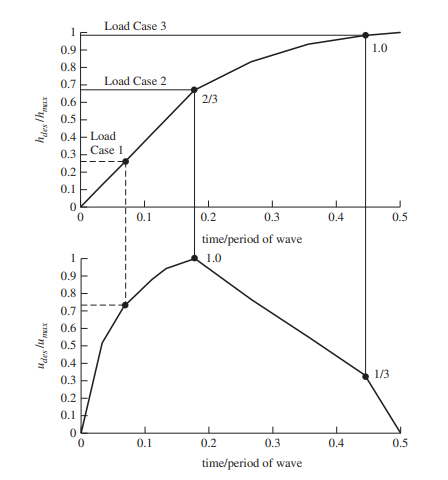
\includegraphics[width=0.6\textwidth]{fig1.png}
\caption{The relationship between inundation height and flow velocity for three cases of tsunami loading \citep{leet}.}
\label{fig:loadcases}
\end{figure}

\subsubsection{Hydrostatic load}
Hydrostatic load is caused by the stationary mass of water. The load due to the hydrostatic force of water is in the form of horizontal and vertical forces from structures submerged in water. Equation \ref{eq:hydrostatic load} describes the horizontal force that results from the hydrostatic pressure of water.

\begin{equation}
F_h= \frac{1}{2} \gamma_s b h_{des}^2
\label{eq:hydrostatic load}
\end{equation}

\noindent where:

\begin{conditions*}
b    &  width of submerged elements\\
h_{des}     &  designed water level \\
\gamma_{s} &  \num{1130}\unit{kg/m^3} (density of seawater, \num{1030}\unit{kg/m^3}, multiplied by 1.1 to account for the sediment and debris in tsunami water)\\
\end{conditions*}

\begin{figure}[H]
\centering
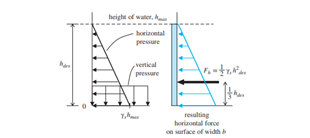
\includegraphics[width=0.6\textwidth]{Picture1.png}
\caption{Hydrostatic pressure due to tsunami inundation \citep{leet}.}
\label{fig:hydrostatic}
\end{figure}

Hydrostatic force can work in vertical and horizontal directions. If the inundation height is above the height of opening in the building, water entering through the opening will remain in the building after the tsunami wave subsides. The magnitude of the additional load on the floor can be expressed as pressure in equation \ref{eq:hydrostatic vertical}.

\begin{equation}
p_r= \gamma_s h_{r}
\label{eq:hydrostatic vertical}
\end{equation}

\noindent where:

\begin{conditions*}
h_r    &  height of the wall above the submerged floor, refer to figure \ref{fig: vertical hydrostatic}\\
\end{conditions*}

Hydrostatic pressure also causes horizontal forces when the tsunami waves subside. The pressure that arises due to water entering the building is shown in figure \ref{fig: vertical hydrostatic}. Vertical pressure can also be seen which provides additional weight to the submerged floor.


\begin{figure}[H]
\centering
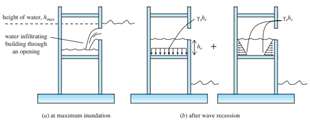
\includegraphics[width=0.6\textwidth]{Picture2.png}
\caption{Pressure due to hydrostatic forces (a) when tsunami reaches its maximum (b) after the wave subsided \citep{leet}.}
\label{fig: vertical hydrostatic}
\end{figure}

Lift can occur if there is empty space that is submerged without openings. The lift force of the structure displacing the volume of water can be expressed by equation \ref{eq:lift}. This is the same as Archimedes’ principle of body submerged in water.

\begin{equation}
F_v= \gamma_s V_w
\label{eq:lift}
\end{equation}

\noindent where:

\begin{conditions*}
V_w    &  the volume of water displaced from the structure\\
\end{conditions*}

\begin{figure}[H]
\centering
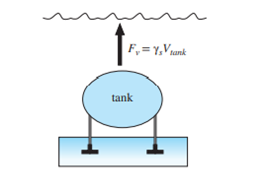
\includegraphics[width=0.5\textwidth]{Picture3.png}
\caption{Lifting force due to volume of water displaced by objects \citep{leet}.}
\label{fig: lifting force}
\end{figure}

\subsubsection{Hydrodynamic load}
Hydrodynamic loads have a principle similar to pressure caused by wind, hydrodynamic loads vary according to speed $u$. The lateral force applied to the lateral force resisting system at each height, $x$, can be calculated by equation \ref{eq:hydrodynamic}.

\begin{equation}
F_{dx}= \frac{1}{2}\rho_s I_{tsu} C_d C_{cx} B h_{des} u_{des}^2
\label{eq:hydrodynamic}
\end{equation}

\noindent where:

\begin{conditions*}
F_{dx}   &  hydrodynamic lateral force applied at level x\\
\rho_{s}   &  specific gravity of tsunami water, \num{1130}\unit{kg/m^3}\\
B & building wall width\\
h_{des} & inundation height\\
u_{des} & corresponding flow rate according to figure \ref{fig:loadcases}\\
I_{tsu} & tsunami importance factor \\
C_d & drag coefficient ratio based on table \ref{tab:dragcoeff} \\
C_{cx} & closure coefficient, refer to equation  \ref{eq:closurecoeff} \\
\end{conditions*}

\renewcommand{\arraystretch}{1}
\begin{longtable}{P{2in} P{2in}}
\caption{Drag coefficient for rectangular structures. Source: \cite{sni172720} and \cite{asce}.}\\

\headrow \thead{Ratio betweeen width and inundation depth, $B/h_{sx}$} & \thead{Drag coefficient, $C_d$}  \\
$<12$ &$1.25$\\
$16$ & $1.30$\\
$26$ & $1.40$\\
$36$ & $1.50$\\
$60$ & $1.75$\\
$100$ & $1.80$\\
$\geq 120$ & $2.00$\\
\label{tab:dragcoeff}
\end{longtable}

The value of the closure coefficient can be assumed to be conservative at 1.0. This value can also be calculated from the ratio of the area of the building elements multiplied by certain factors compared to the total area which is the width multiplied by the inundation height. The formula is expressed mathematically as equation \ref{eq:closurecoeff}.

\begin{equation}
C_{cx}= \frac{\sum(A_{col}+A_{wall})+1.5 \times A_{beam}}{B \times h_{sx}}\label{eq:closurecoeff}
\end{equation}

The areas of the columns and walls are the vertical projections of the columns and walls. The area of the beam is the largest beam exposed to flow laterally. This sum is divided by the width of the entire wall, $B$, multiplied by the average story height, $h_{sx}$.  The closure coefficient, $C_{cx}$, taken need not be more than \num{1.00}.

\subsubsection{Debris impact load}
ASCE and SNI standards provide a simple equation for calculating debris impact loads. The impact load can be taken in value as equations \ref{eq:dlkips} or \ref{eq:dlkn}.

\begin{equation}
F_{i} = 330 \times C_o \times I_{tsu} (kips)
\label{eq:dlkips}
\end{equation}

\begin{equation}
F_{i} = \num{1470}  \times C_o \times I_{tsu} (kN)
\label{eq:dlkn}
\end{equation}

\noindent where:

\begin{conditions*}
C_0 & 0,65, is the orientation coefficient of the debris which represents the probability of debris not hitting the building perpendicularly\\
I_{tsu} & tsunami importance factor \\
\end{conditions*}

\subsection{Earthquake Load}
Earthquake load are caused by ground movements that cause buildings to change suddenly. This movement causes a deflection in the building, due to the inertia of the building. This causes an internal force due to the deflection as shown in figure \ref{fig:deflected quake}.

\begin{figure}[H]
\centering
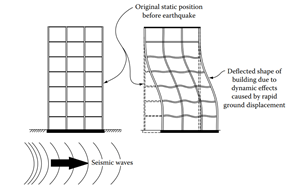
\includegraphics[width=0.5\textwidth]{Picture4.png}
\caption{Displacement of buildings caused by earthquake \citep{taranath}.}
\label{fig:deflected quake}
\end{figure}

Earthquake load has been adopted in the SNI 1726:2019 standard. Maximum considered earhquake is probability of the value being exceeded in magnitude for 50 years by \SI{2}{\percent}. The considered earthquake has an effective return period of 2475 years.\label{2475} The method of response spectrum analysis for applying earthquake forces in accordance with SNI 1726:2019 are given in \ref{subsub: eqimportance} to \ref{subsub: appresponsespectrum}.

\subsubsection{Determining earthquake importance factor}
\label{subsub: eqimportance}
Importance factor of the earthquake shows the relative importance of the building based on its function and use. Conceptually, it represents the expected building performance during and after an earthquake. The increase in base shear depends on the risk category of the building, where for risk category III it is increased by \SI{25}{\percent} and \SI{50}{\percent} for risk category IV which can be seen in table \ref{tab:prioreq} \citep{taranath}.

\renewcommand{\arraystretch}{1}
\begin{longtable}{P{2in} P{2in}}
\caption{Importance factor of earthquake. Source: \cite{sni172619}.}\\
\headrow \thead{Risk category} & \thead{Earthquake importance factor, $I_e$}  \\
I or II &$1.00$\\
III & $1.25$\\
IV & $1.50$\\
\label{tab:prioreq}
\end{longtable}

\subsubsection{Site classification}
Site class is determined by the top 30 m (100 ft) of soil characteristics. Site classes are divided into several categories, including SA (hard rock), SB (rock), SC (hard, very dense soil and soft rock), SD (medium soil), SE (soft soil) and SF (special soil, which requires specific geotechnical investigations).

\subsubsection{Earthquake parameter determination}
\label{subsub:eqparam}
Earthquake parameters are obtained according to the location of the structure. Parameters $S_s$ and $S_1$ indicate the parameters of the earthquake acceleration in the short period (0.2 seconds) and the 1-second period and are considered with a damping ratio of \SI{5}{\percent}. The value of this parameter can be seen in the attachment to SNI 1726:2019 or through the Puskim PUPR website or application for Indonesia region. This value will later become the basis for determining the base shear force of the earthquake. The typical earthquake response spectrum graphics for ASCE and SNI standards is given in figure \ref{fig:respspectra}.

\begin{figure}[H]
\centering
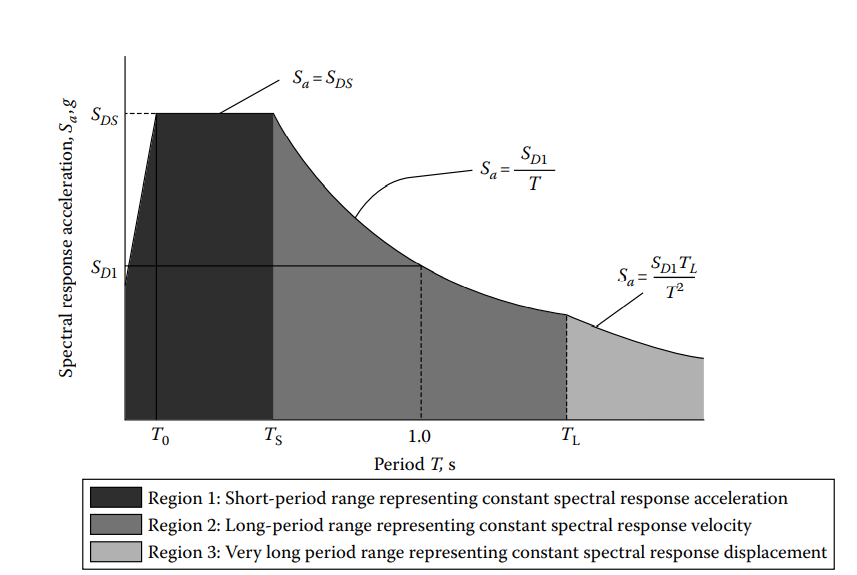
\includegraphics[width=0.6\textwidth]{fig2.png}
\caption{Response spectrum according to ASCE 7-16 or SNI 1726:2019 \citep{taranath}.}
\label{fig:respspectra}
\end{figure}

Site class affects the amplification factor on the value of $S_s$ and $S_1$. This value is an adjustment factor based on site class $F_a$ (short-period site coefficient, 0.2 seconds) and $F_v$ (long-period site coefficient, 1 second). As has been described in \ref{2475} that the considered earthquake is with a return period of 2475 years. This earthquake force is then reduced with a probability of exceeding \SI{10}{\percent} in 50 years, so the return period is 475 years. This also means that earthquake forces that exceed the design within 1 year are likely to occur by \SI{0.2105}{\percent}. The parameters are reduced to $S_{DS}$ and $S_{D1}$ where subscript D represents the designed earthquake.

\subsubsection{Seismic design category determination}
Seismic design category will determine how severe the effect of the earthquake is on the building being reviewed. The determination of the seismic design category depends on the size of the seismic design parameters and importance factor of the building defined in \ref{subsub:eqparam} and \ref{subsub: eqimportance} respectively. The seismic design category will determine the allowable structural system and load combination requirements and what needs to be done if there is structural irregularity.

\subsubsection{Structural system determination}
The structural system is selected for each building axis. Structures may be designed inelastic at the time of experiencing an earthquake. The selection of the type of structure is adjusted to the requirements of SNI 1726:2019. Structures have 3 factors as a conversion from inelastic analysis to elastic analysis. These factors are $R$ (response modification coefficient), $C_d$ (overstrength factor) and $\Omega_0$ (lateral drift amplification factor). Figure \ref{fig:structural factors} shows an illustration to determine structural systems and its corresponding factors.

\begin{figure}[H]
\centering
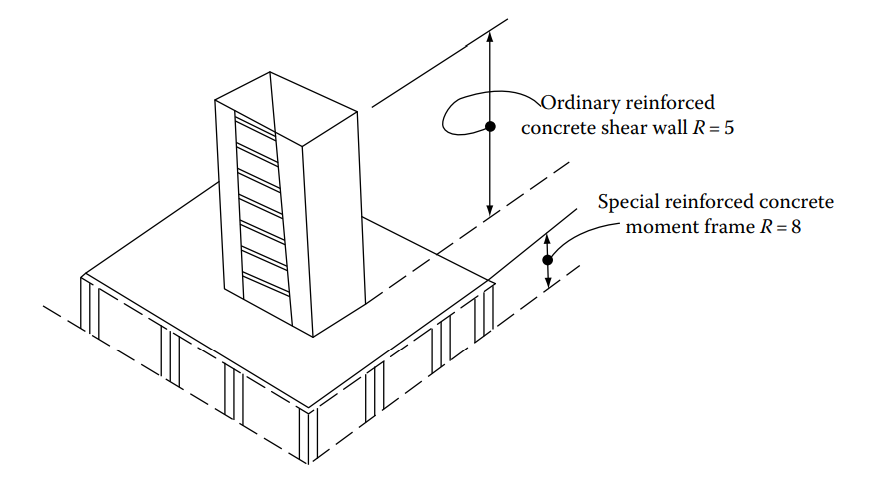
\includegraphics[width=0.6\textwidth]{fig3.png}
\caption{Structural factors determination \citep{taranath}.}
\label{fig:structural factors}
\end{figure}

\subsubsection{Calculation of structure period}
The period of the structure is obtained from the structure analysis program with the upper limit $C_uT_a$ where $T_a$ is the approximate fundamental period and $C_u$ is the coefficient of the upper limit whose value depends on the design spectral response acceleration parameter of 1 second-period, $S_{D1}$, which are given in table \ref{tab:cu}. The approximate fundamental period can be calculated by equation \ref{eq:fundamentalperiod}.

\begin{equation}
T_{a} = C_t \times h_n^x
\label{eq:fundamentalperiod}
\end{equation}

\noindent where:

\begin{conditions*}
h_n    &  structure height (m)\\
C_t & coefficient defined in table \ref{tab:ctx} \\
x & coefficient defined in table \ref{tab:ctx}
\end{conditions*}

\makeatletter
\newcommand\footnoteref[1]{\protected@xdef\@thefnmark{\ref{#1}}\@footnotemark}
\makeatother

\renewcommand{\arraystretch}{1}
\begin{longtable}{P{2.5in} P{1in} P{1in}}
\caption{Value of approximate period parameter. Source: \cite{sni172720} and \cite{asce}.}\\
\headrow \thead{Structure type} & \thead{$C_t$} & \thead{x} \\
Steel moment-resisting frames \footnote{\label{foot:period}Moment-resisting frame systems that resist \SI{100}{\percent} loads and not adjoined with other structural components that will prevent the frames to be deflected when experiencing earthquakes.} &$0.028 (0.0724)$\footnote{\label{foot:metric} Metric values are given in parantheses.}  & $0.8$\\
Concrete moment-resisting frames \footnoteref{foot:period} &$0.016 (0.0466)$\footnoteref{foot:metric}  & $0.9$\\
Steel eccentricaly braced frames &$0.03 (0.0731)$\footnoteref{foot:metric}  & $0.75$\\
Steel buckling-restrained braced frames &$0.03 (0.0731)$\footnoteref{foot:metric}  & $0.75$\\
All other structural systems &$0.02 (0.0488)$\footnoteref{foot:metric}  & $0.75$\\
\label{tab:ctx}
\end{longtable}


\renewcommand{\arraystretch}{1}
\begin{longtable}{P{1in} P{1in}}
\caption{Value of upper limit coefficient to calculate fundamental period. Source: \cite{sni172720} and \cite{asce}.}\\
\headrow \thead{$S_{D1}$} & \thead{$C_u$}  \\
$\geq 0.4$ & $1.4$ \\
$0.3$ & $1.4$ \\
$0.2$ & $1.5$ \\
$0.15$ & $1.6$ \\
$\leq 0.1$ & $1.7$ \\
\label{tab:cu}
\end{longtable}

\subsubsection{Calculation of base shear force}
The base shear force will determine the amount of lateral force to be applied to the building, which is proportional to the effective seismic weight. The seismic base shear force is calculated by equation \ref{eq:baseshear}.

\begin{equation}
V = C_s \times W
\label{eq:baseshear}
\end{equation}

\noindent where:

\begin{conditions*}
C_s    &  seismic response coefficient\\
W & seismic weight \\
\end{conditions*}

\subsubsection{Response spectrum application}
\label{subsub: appresponsespectrum}
Response spectrum is a method that uses a combination of mass in determining maximum response due to earthquake loads on structures. The modal mass participation factor is at least 90 percent for each orthogonal horizontal direction of the structure under review. If the combined base shear force, $V_t$, is less than \SI{100}{\percent} of the base shear force calculated using the lateral equivalent force, $V$, then the force needs to be scaled with the ratio of these two.

\section{Methodology}
\label{sec:method}

Research flowchart used in this study can be seen in figure \ref{fig: flowchart}. The research was carried out to determine the structure's response to variations in tsunami loading and to assess whether the structure with current seismic criteria could withstand the design forces of tsunami. The comparison was made to structural response such as internal forces and deflections.

The structure chosen was a 10-story office building with a base story height of 4 meters and typical floors of 3.5 meters. In both directions the span of the beam was 4 meters, there were 4 beams in the y direction and 8 beams in the x direction. Plan and elevation views are given in figure \ref{fig:plan} and \ref{fig:elevation} respectively.

The building was designed as an office building which was a category II facility for earthquake loads and category III for tsunami loads. The masonry for the tsunami retained water calculations was at 90 cm above the floor slab. The highest elevation of the window is 120 cm above the masonry as shown in figure \ref{fig:masonry}.

\begin{figure}[H]
\centering
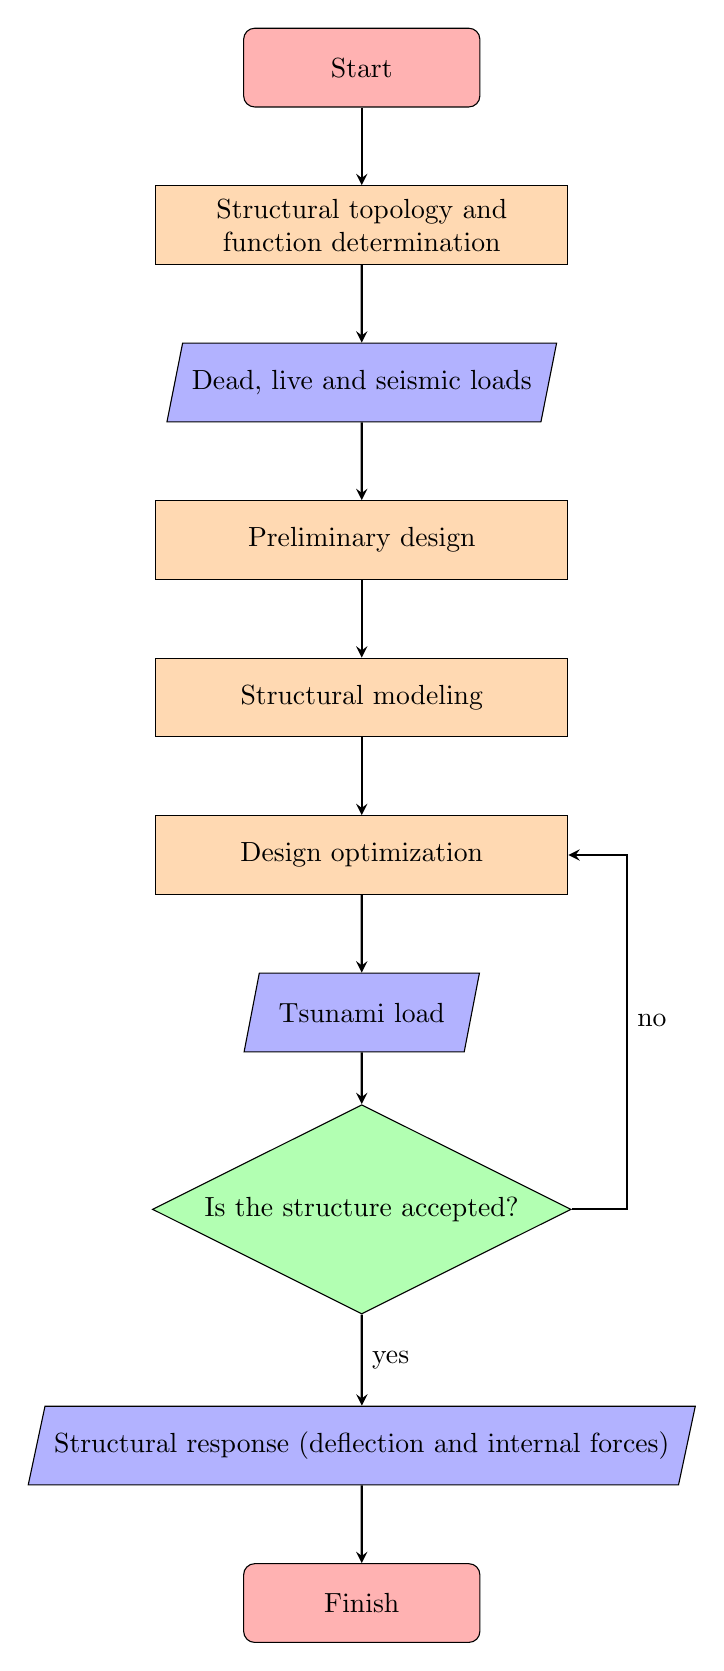
\begin{tikzpicture}[node distance=2cm]

\node (start) [startstop] {Start};
\node (in1) [process, below of=start] {Structural topology and function determination};
\node (pro1) [io, below of=in1] {Dead, live and seismic loads};

\node (pro2) [process, below of=pro1] {Preliminary design};
\node (pro3) [process, below of=pro2] {Structural modeling};
\node (pro4) [process, below of=pro3] {Design optimization};
\node (pro5) [io, below of=pro4] {Tsunami load};
\node (dec1) [decision, below of=pro5, yshift=-0.5cm] {Is the structure accepted?};

%\node (pro2a) [process, below of=dec1, yshift=-0.5cm] {Process 2a
%text text text text
%text text text 
%text text text};

%\node (pro2b) [process, right of=dec1, xshift=2cm] {Process 2b};
\node (out1) [io, below of=dec1, yshift=-1cm] {Structural response (deflection and internal forces)};
\node (stop) [startstop, below of=out1] {Finish};

\draw [arrow] (start) -- (in1);
\draw [arrow] (in1) -- (pro1);
\draw [arrow] (pro1) -- (pro2);
\draw [arrow] (pro2) -- (pro3);
\draw [arrow] (pro3) -- (pro4);
\draw [arrow] (pro4) -- (pro5);
\draw [arrow] (pro5) -- (dec1);
\draw [arrow] (dec1) -- node[anchor=south, midway, right] {yes} (out1);
\draw [arrow] (dec1.east) |- +(20pt,0pt) |- node[anchor=east, right, yshift=-60pt] {no} (pro4.east);
%\draw [arrow] (pro2) |- (pro1);
%\draw [arrow] (pro2a) -- (out1);
\draw [arrow] (out1) -- (stop);

\end{tikzpicture}

\caption{Research flowchart.}
\label{fig: flowchart}
\end{figure}

\begin{figure}[H]
\centering
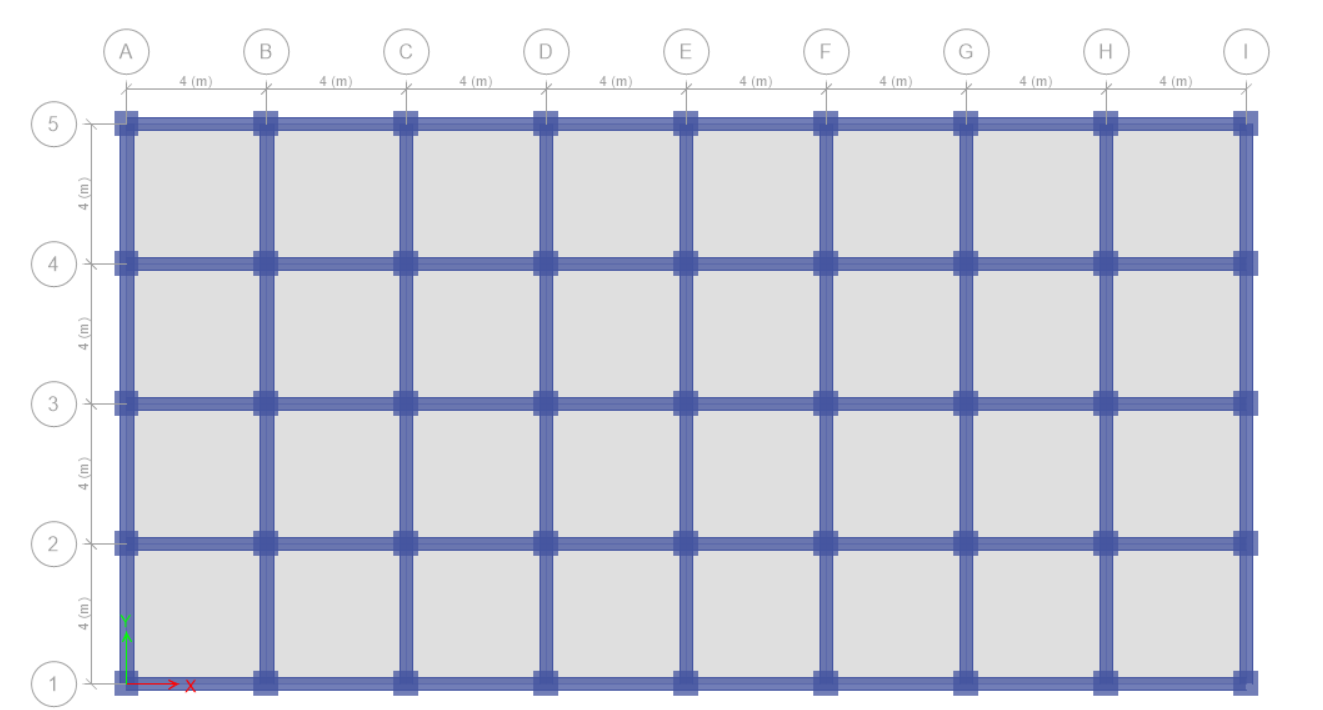
\includegraphics[width=0.6\textwidth]{fig4.png}
\caption{Plan view of structure used.}
\label{fig:plan}
\end{figure}

\begin{figure}[H]
\begin{minipage}{0.4\textwidth}
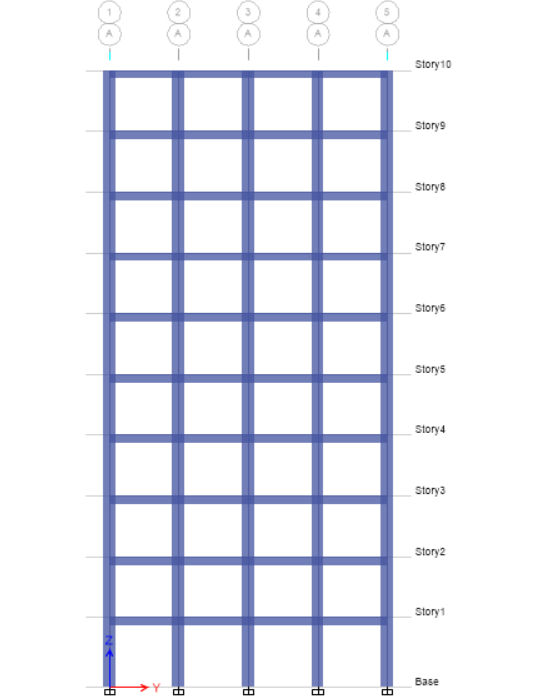
\includegraphics[width=\linewidth]{fig5.png}
\subcaption{YZ elevation view.}
\end{minipage}
\hfill
\begin{minipage}{0.6\textwidth}
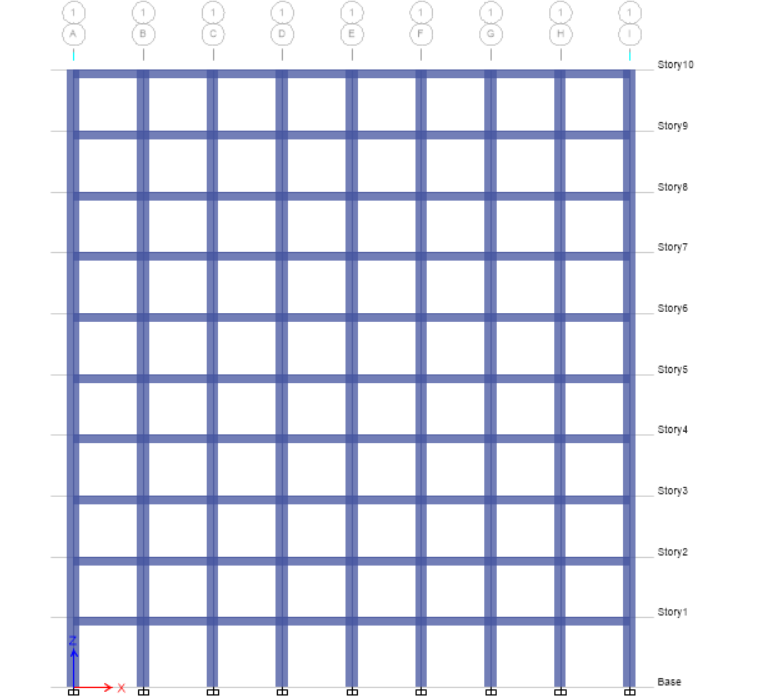
\includegraphics[width=\linewidth]{fig6.png}
\subcaption{XZ elevation view.}
\end{minipage}

\caption{Elevation views of structure used.}
\label{fig:elevation}
\end{figure}

\begin{figure}[H]
\centering
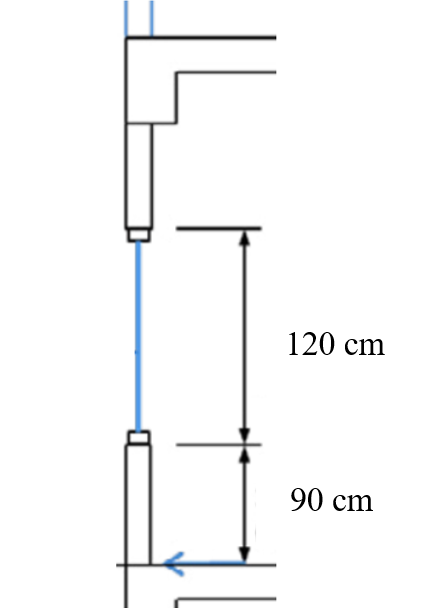
\includegraphics[width=0.35\textwidth]{fig7.png}
\caption{Elevation of masonry and window \citep{rob}.}
\label{fig:masonry}
\end{figure}

The concrete quality were in the range of 30-50 MPa. The concrete reinforcement yield strength was, $f_y$ = $400$ MPa. The building system was designed with special moment resisting frame system criteria which is considered economical for up to 25 floors \citep{taranath}. This also considers the reduction of the tsunami load due to removal of structural walls.

The following were brief steps of the research that has been done:
\begin{enumerate}
\item{The building was designed to resist dead, live and earthquake loads.}
\item{The building resulting from the initial design was loaded with varying tsunami loads and adjusted accordingly.}
\item{The results of the first step of the building design were compared with the second step. The comparison includes deformation, internal forces and structural weight.}
\end{enumerate}

In the second step, the height of the tsunami varied from one to three floors, with an increment of one floor. Tsunamis were subjected perpendicular to the broad side of the building (The tsunami direction was parallel to Y axis in figure \ref{fig:plan}). Variations were made to the acceptance criteria for the structure, namely linear criteria and nonlinear criteria. These acceptance criteria were based on article 6.8.3.5 of SNI 1727:2020 which allows these two criteria to be selected as structural design guidelines. The variations in tsunami height and acceptance criteria were combined, thus there were 7 models that were analyzed which are summarized in table \ref{tab:model definition}.

\renewcommand{\arraystretch}{1}
\begin{longtable}{P{0.5in} P{1in} P{2in} P{1in} P{1in}}
\caption{Model definition.}\\
\headrow \thead{Model} & \thead{Tsunami height} & \thead{Tsunami load acceptance criteria} & \thead{Information} \\
1 & -&-& control model \\
2 & 1 floor&Linear analysis& - \\
3 & 1 floor&Nonlinear analysis& - \\
4 & 2 floors&Linear analysis& - \\
5 & 2 floors&Nonlinear analysis& -\\
6 & 3 floors&Linear analysis& -\\
7 & 3 floors&Nonlinear analysis& - \\
\label{tab:model definition}
\end{longtable}

This study used fixed variables in the form of material quality, structural topology (relationships between structural elements), and loading other than tsunami. The independent variables that varied were the tsunami loading and the acceptance criteria for the structure. Comparisons were made to the dependent variables, namely deformation, internal force and structural weight. 

\section{Results and discussion}
\label{sec:results}

Earthquakes model structural design was carried out by using heuristic optimization. Design optimization is done by adjusting the member sizes to the behavior of the structure. The structural member size results to resist earthquake load according to the Banda Aceh spectrum response with soft soil conditions are given in figures \ref{fig:XZ view} and \ref{fig:YZ view}.

\begin{figure}[H]
\centering
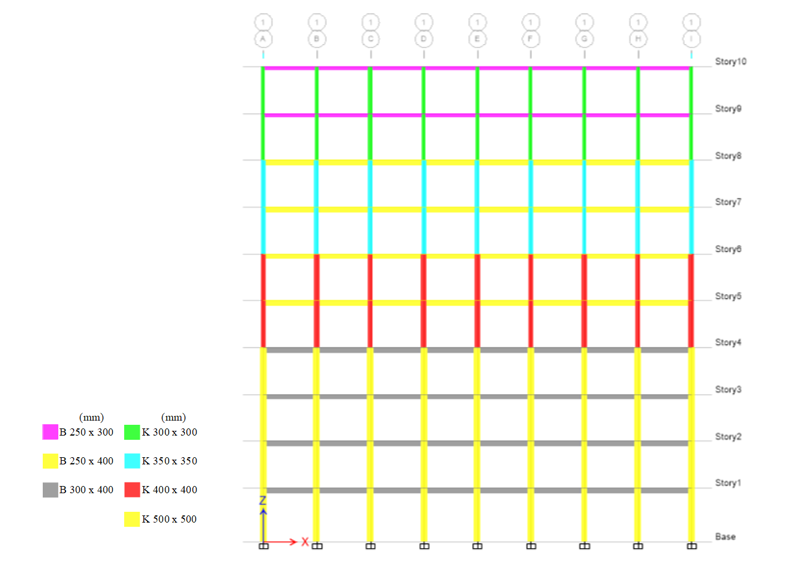
\includegraphics[width=0.6\textwidth]{Picture6.png}
\caption{XZ elevation view of the design result.}
\label{fig:XZ view}
\end{figure}

\begin{figure}[H]
\centering
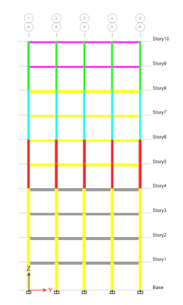
\includegraphics[width=0.3\textwidth]{Picture7.png}
\caption{YZ elevation view of the design result.}
\label{fig:YZ view}
\end{figure}

The structure was designed to have typical beams and columns for one floor. A summary of the cross-section of the building per floor can be seen in table \ref{tab:cross section model 1}. The building has a structural weight of, $W_{structure}=\num{27652,93} \si{kN}$. The base shear force for the seismic load in Banda Aceh for that particular structure was, $E_h=\num{2988,62} \si{kN}$.

%\begin{table}[H]
\renewcommand{\arraystretch}{1}
%\centering
\begin{longtable}{P{0.75in} P{1.25in} P{1.25in} P{1.25in}}
\caption{Summary of structural elements in model 1 (earthquake loads only).}\\
\headrow \thead{Floor} & \thead{Beam cross section (mm)} & \thead{Column cross section (mm)} & \thead{Structure weight (kN)} \\
1 & $300 \times 400$ & $500 \times 500$ & \num{3256.43}  \\
2 & $300 \times 400$ & $500 \times 500$ & \num{3124.04}  \\
3 & $300 \times 400$ & $500 \times 500$ & \num{3124.04}  \\
4 & $300 \times 400$ & $500 \times 500$ & \num{3124.04}  \\
5 & $250 \times 400$ & $400 \times 400$ & \num{2683.10}  \\
6 & $250 \times 400$ & $400 \times 400$ & \num{2683.10}  \\
7 & $250 \times 400$ & $350 \times 350$ & \num{2553.03}  \\
8 & $250 \times 400$ & $350 \times 350$ & \num{2553.03}  \\
9 & $250 \times 300$ & $300 \times 300$ & \num{2276.04}  \\
10 & $250 \times 300$ & $300 \times 300$ & \num{2276.04}  \\
 &  & Total structural weight & \num{27652.93}  \\
\label{tab:cross section model 1}
\end{longtable}
%\end{table}  

Drifts evaluation were performed for seismic forces with and without induced torsion for each of the direction. The induced torque is given from an eccentricity of \SI{5}{\percent} of the size of the diaphragm perpendicular to the seismic force for each direction. The drift calculation results for each load case are presented in figure \ref{fig:driftchecking}.

\begin{figure}[H]
\centering
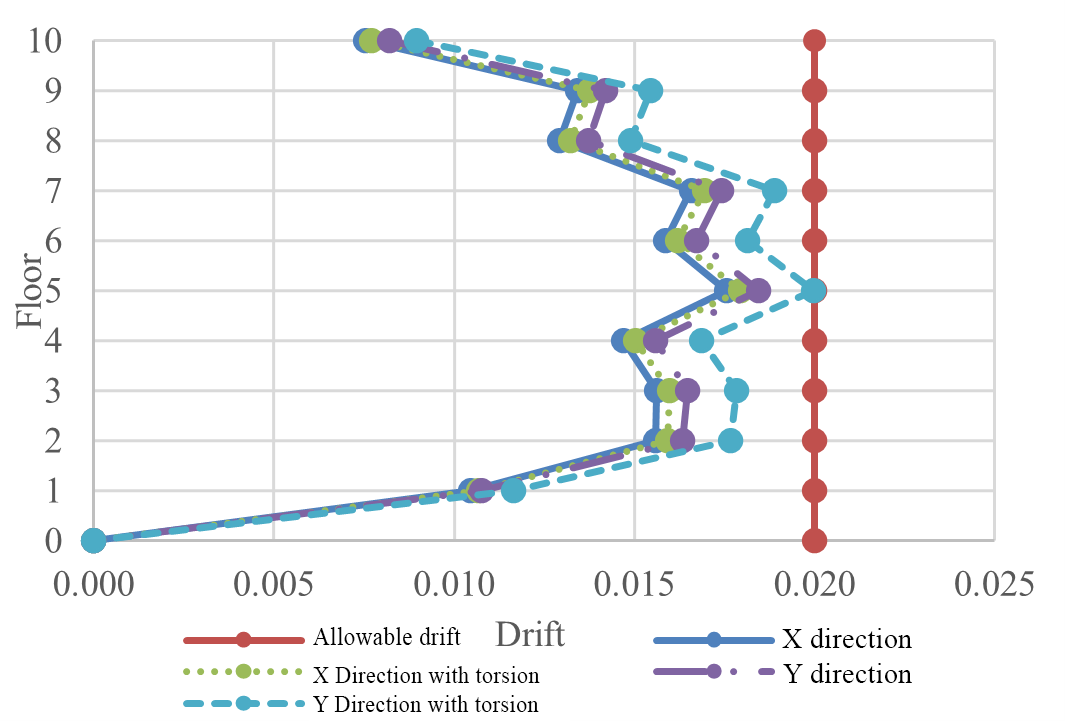
\includegraphics[width=0.7\textwidth]{Picture8_engels.png}
\caption{Drift checking in earthquake model (model 1).}
\label{fig:driftchecking}
\end{figure}

Structures that were built to withstand seismic forces had their designs tested for tsunami loading. A summary of the tsunami force calculations for load cases 1, 2 and 3 in accordance with figure \ref{fig:loadcases} can be seen in figures \ref{fig:lc1}, \ref{fig:lc2} and \ref{fig:lc3}. These loads were applied to each floor.

\begin{figure}[H]
\centering
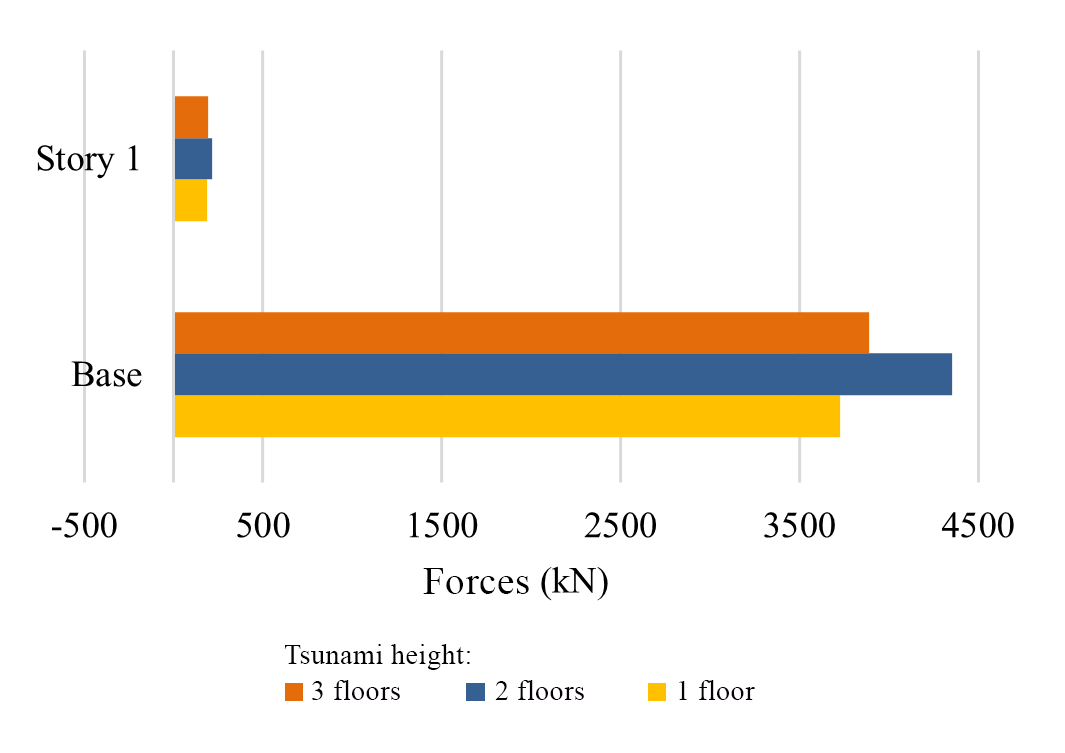
\includegraphics[width=0.5\textwidth]{Picture9_engels.png}
\caption{Tsunami forces for load case 1.}
\label{fig:lc1}
\end{figure}

\begin{figure}[H]
\centering
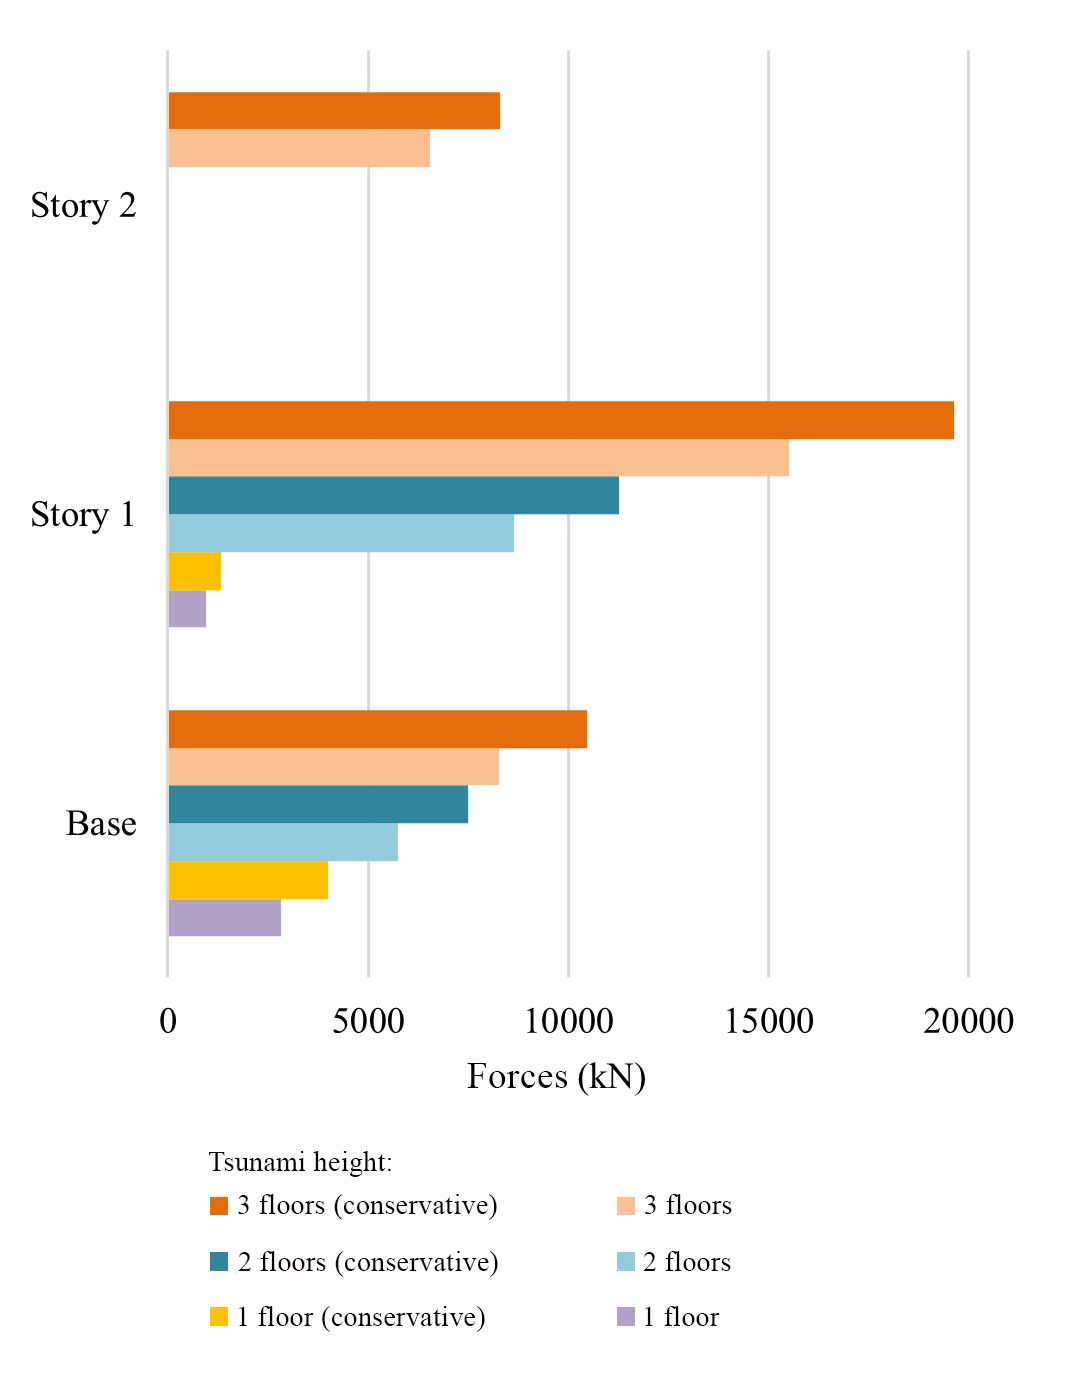
\includegraphics[width=0.5\textwidth]{Picture10_engels.png}
\caption{Tsunami forces for load case 2.}
\label{fig:lc2}
\end{figure}

\begin{figure}[H]
\centering
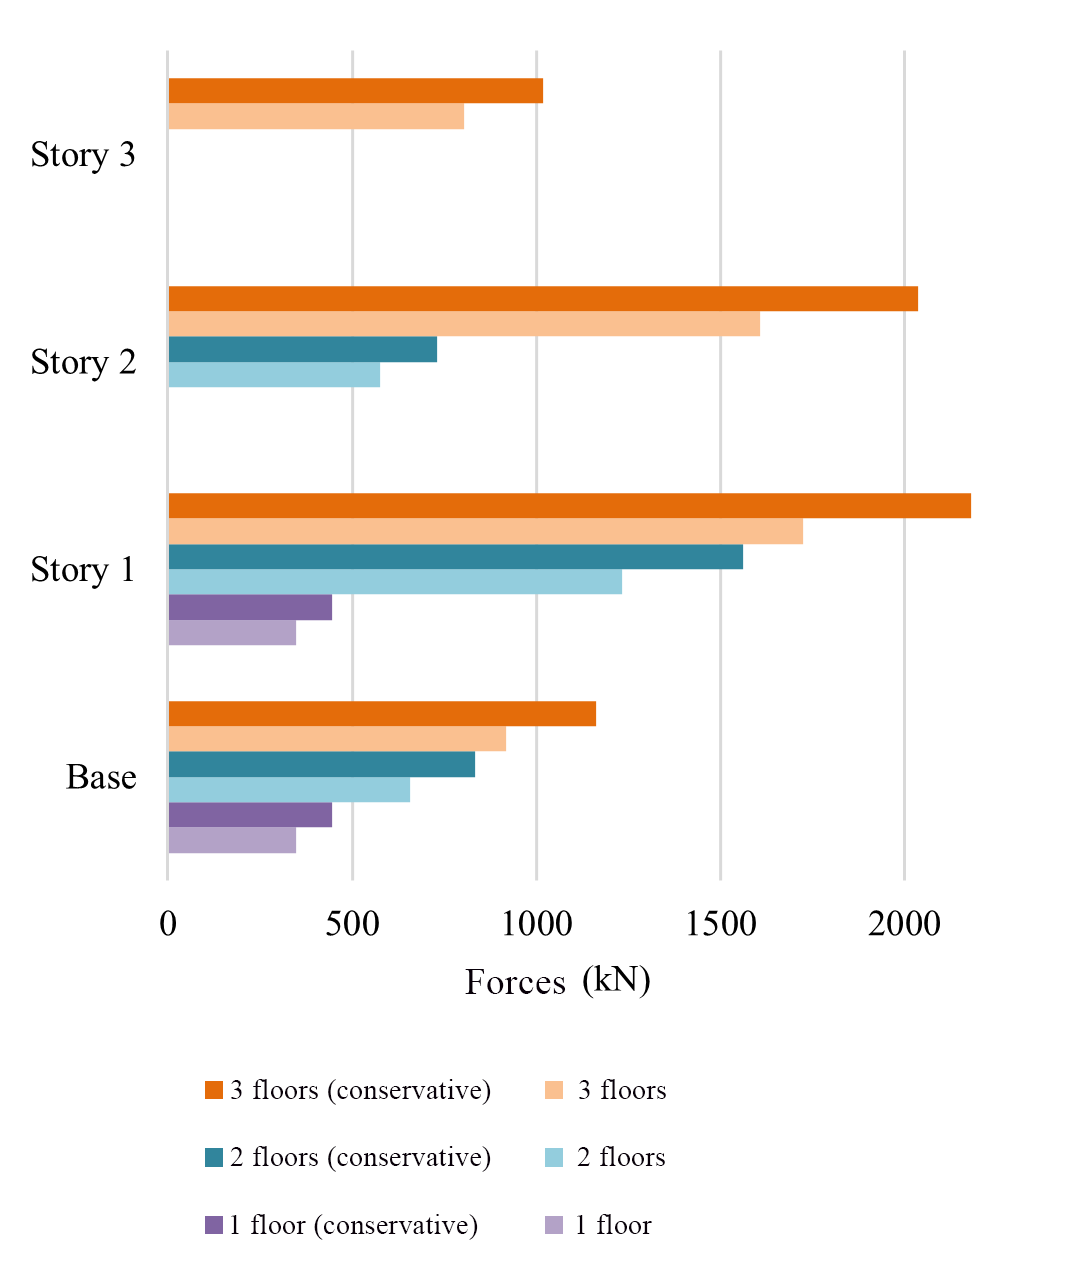
\includegraphics[width=0.5\textwidth]{Picture11_engels.png}
\caption{Tsunami forces for load case 3.}
\label{fig:lc3}
\end{figure}

The structure of model 1, in table \ref{tab:cross section model 1} was loaded with each load case within each model and optimized to resist the loads with the corresponding structural acceptance criteria according to table \ref{tab:model definition}. The results of structural optimization for each tsunami load model can be seen from table \ref{tab:cross section model 2} to \ref{tab:cross section model 7}.

\renewcommand{\arraystretch}{1}
\begin{longtable}{P{0.5in} P{1in} P{1in} P{1in} P{1in}}
\caption{Summary of structural elements in model 2.}\\
\headrow \thead{Floor} & \thead{Interior column (mm)} & \thead{Exterior column (mm)} & \thead{Beam (mm)} & \thead{Structure weight (kN)} \\
1 & $500 \times 500$ & $600 \times 600$ & $300 \times 400$ & \num{3495.37} \\
2 & $500 \times 500$ & $500 \times 500$ & $300 \times 400$ & \num{3124.04} \\
3 & $500 \times 500$ & $500 \times 500$ & $300 \times 400$ & \num{3124.04} \\
4 & $500 \times 500$ & $500 \times 500$ & $300 \times 400$ & \num{3124.04} \\
5 & $400 \times 400$ & $400 \times 400$ & $250 \times 400$ & \num{2683.10} \\
6 & $400 \times 400$ & $400 \times 400$ & $250 \times 400$ & \num{2683.10} \\
7 & $350 \times 350$ & $350 \times 350$ & $250 \times 400$ & \num{2553.03} \\
8 & $350 \times 350$ & $350 \times 350$ & $250 \times 400$ & \num{2553.03} \\
9 & $300 \times 300$ & $300 \times 300$ & $250 \times 300$ & \num{2276.04} \\
10 & $300 \times 300$ & $300 \times 300$ & $250 \times 300$ & \num{2276.04} \\
 &  & & Total structural weight & \num{27891.86} \\
\label{tab:cross section model 2}
\end{longtable}

\renewcommand{\arraystretch}{1}
\begin{longtable}{P{0.5in} P{1in} P{1in} P{1in} P{1in}}
\caption{Summary of structural elements in model 3.} \\
\headrow \thead{Floor} & \thead{Interior column (mm)} & \thead{Exterior column (mm)} & \thead{Beam (mm)} & \thead{Structure weight (kN)} \\
1 & $500 \times 500$ & $550 \times 550$ & $300 \times 400$ & \num{3370.25} \\
2 & $500 \times 500$ & $500 \times 500$ & $300 \times 400$ & \num{3124.04} \\
3 & $500 \times 500$ & $500 \times 500$ & $300 \times 400$ & \num{3124.04} \\
4 & $500 \times 500$ & $500 \times 500$ & $300 \times 400$ & \num{3124.04} \\
5 & $400 \times 400$ & $400 \times 400$ & $250 \times 400$ & \num{2683.10} \\
6 & $400 \times 400$ & $400 \times 400$ & $250 \times 400$ & \num{2683.10} \\
7 & $350 \times 350$ & $350 \times 350$ & $250 \times 400$ & \num{2553.03} \\
8 & $350 \times 350$ & $350 \times 350$ & $250 \times 400$ & \num{2553.03} \\
9 & $300 \times 300$ & $300 \times 300$ & $250 \times 300$ & \num{2276.04} \\
10 & $300 \times 300$ & $300 \times 300$ & $250 \times 300$ & \num{2276.04} \\
 &  & & Total structural weight & \num{27766.74} \\
\label{tab:cross section model 3}
\end{longtable}

\renewcommand{\arraystretch}{1}
\begin{longtable}{P{0.5in} P{1in} P{1in} P{1in} P{1in}}
\caption{Summary of structural elements in model 4.}\\
\headrow \thead{Floor} & \thead{Interior column (mm)} & \thead{Exterior column (mm)} & \thead{Beam (mm)} & \thead{Structure weight (kN)} \\
1 & $650 \times 650$ & $1000 \times 1000$ & $350 \times 500$ & \num{5540.42} \\
2 & $500 \times 500$ & $550 \times 550$ & $300 \times 400$ & \num{3223.03} \\
3 & $500 \times 500$ & $500 \times 500$ & $300 \times 400$ & \num{3124.04} \\
4 & $500 \times 500$ & $500 \times 500$ & $300 \times 400$ & \num{3124.04} \\
5 & $400 \times 400$ & $400 \times 400$ & $250 \times 400$ & \num{2683.10} \\
6 & $400 \times 400$ & $400 \times 400$ & $250 \times 400$ & \num{2683.10} \\
7 & $350 \times 350$ & $350 \times 350$ & $250 \times 400$ & \num{2553.03} \\
8 & $350 \times 350$ & $350 \times 350$ & $250 \times 400$ & \num{2553.03} \\
9 & $300 \times 300$ & $300 \times 300$ & $250 \times 300$ & \num{2276.04} \\
10 & $300 \times 300$ & $300 \times 300$ & $250 \times 300$ & \num{2276.04} \\
 &  & & Total structural weight & \num{30035.91} \\
\label{tab:cross section model 4}
\end{longtable}

\renewcommand{\arraystretch}{1}
\begin{longtable}{P{0.5in} P{1in} P{1in} P{1in} P{1in}}
\caption{Summary of structural elements in model 5.}\\
\headrow \thead{Floor} & \thead{Interior column (mm)} & \thead{Exterior column (mm)} & \thead{Beam (mm)} & \thead{Structure weight (kN)} \\
1 & $650 \times 650$ & $650 \times 650$ & $300 \times 400$ & \num{3124.04} \\
2 & $500 \times 500$ & $550 \times 550$ & $300 \times 400$ & \num{3223.03} \\
3 & $500 \times 500$ & $500 \times 500$ & $300 \times 400$ & \num{3124.04} \\
4 & $500 \times 500$ & $500 \times 500$ & $300 \times 400$ & \num{3124.04} \\
5 & $400 \times 400$ & $400 \times 400$ & $250 \times 400$ & \num{2683.10} \\
6 & $400 \times 400$ & $400 \times 400$ & $250 \times 400$ & \num{2683.10} \\
7 & $350 \times 350$ & $350 \times 350$ & $250 \times 400$ & \num{2553.03} \\
8 & $350 \times 350$ & $350 \times 350$ & $250 \times 400$ & \num{2553.03} \\
9 & $300 \times 300$ & $300 \times 300$ & $250 \times 300$ & \num{2276.04} \\
10 & $300 \times 300$ & $300 \times 300$ & $250 \times 300$ & \num{2276.04} \\
 &  & & Total structural weight & \num{28450.52} \\
\label{tab:cross section model 5}
\end{longtable}

\renewcommand{\arraystretch}{1}
\begin{longtable}{P{0.5in} P{1in} P{1in} P{1in} P{1in}}
\caption{Summary of structural elements in model 6.}\\
\headrow \thead{Floor} & \thead{Interior column (mm)} & \thead{Exterior column (mm)} & \thead{Beam (mm)} & \thead{Structure weight (kN)} \\
1 & $900\times900$ & $900\times1400$ & $400\times600$ & \num{7182.79} \\
2 & $800\times800$ & $800\times800$ & $400\times600$ & \num{5192.22} \\
3 & $500\times500$ & $550\times550$ & $300\times400$ & \num{3223.03} \\
4 & $500\times500$ & $500\times500$ & $300\times400$ & \num{3124.04} \\
5 & $400\times400$ & $400\times400$ & $250\times400$ & \num{2683.10} \\
6 & $400\times400$ & $400\times400$ & $250\times400$ & \num{2683.10} \\
7 & $350\times350$ & $350\times350$ & $250\times400$ & \num{2553.03} \\
8 & $350\times350$ & $350\times350$ & $250\times400$ & \num{2553.03} \\
9 & $300\times300$ & $300\times300$ & $250\times300$ & \num{2276.04} \\
10 & $300\times300$ & $300\times300$ & $250\times300$ & \num{2276.04} \\
 &  & & Total structural weight & \num{33746.46} \\
\label{tab:cross section model 6}
\end{longtable}

\renewcommand{\arraystretch}{1}
\begin{longtable}{P{0.5in} P{1in} P{1in} P{1in} P{1in}}
\caption{Summary of structural elements in model 7.}\\
\headrow \thead{Floor} & \thead{Interior column (mm)} & \thead{Exterior column (mm)} & \thead{Beam (mm)} & \thead{Structure weight (kN)} \\
1 & $900\times900$ & $900\times900$ & $300\times400$ & \num{5543.00} \\
2 & $700\times700$ & $700\times700$ & $300\times400$ & \num{3970.77} \\
3 & $500\times500$ & $550\times550$ & $300\times400$ & \num{3223.03} \\
4 & $500\times500$ & $500\times500$ & $300\times400$ & \num{3124.04} \\
5 & $400\times400$ & $400\times400$ & $250\times400$ & \num{2683.10} \\
6 & $400\times400$ & $400\times400$ & $250\times400$ & \num{2683.10} \\
7 & $350\times350$ & $350\times350$ & $250\times400$ & \num{2553.03} \\
8 & $350\times350$ & $350\times350$ & $250\times400$ & \num{2553.03} \\
9 & $300\times300$ & $300\times300$ & $250\times300$ & \num{2276.04} \\
10 & $300\times300$ & $300\times300$ & $250\times300$ & \num{2276.04} \\
 &  & & Total structural weight & \num{30885.21} \\
\label{tab:cross section model 7}
\end{longtable}

In Figure \ref{fig:base shear} it can be seen that for models 2 and 3 the tsunami base shear force that occurs was smaller than the seismic base shear force with an overstrength factor. This was consistent with the results of structural analysis, where the dimensional changes in the exterior columns were only caused by local forces which were the debris impact loads. The moment resisting system for models 2 and 3 did not need to be changed from model 1 to withstand a tsunami load as high as 1 floor. Changes were made due to local tsunami loads in the form of local hydrodynamic forces and debris impact loads. In model 4 the tsunami base shear force that occurs exceeds the capacity resulting from the seismic base shear force with an overstrength factor, thus it was necessary to change the dimensions of the lateral force resisting systems.

\begin{figure}[H]
\centering
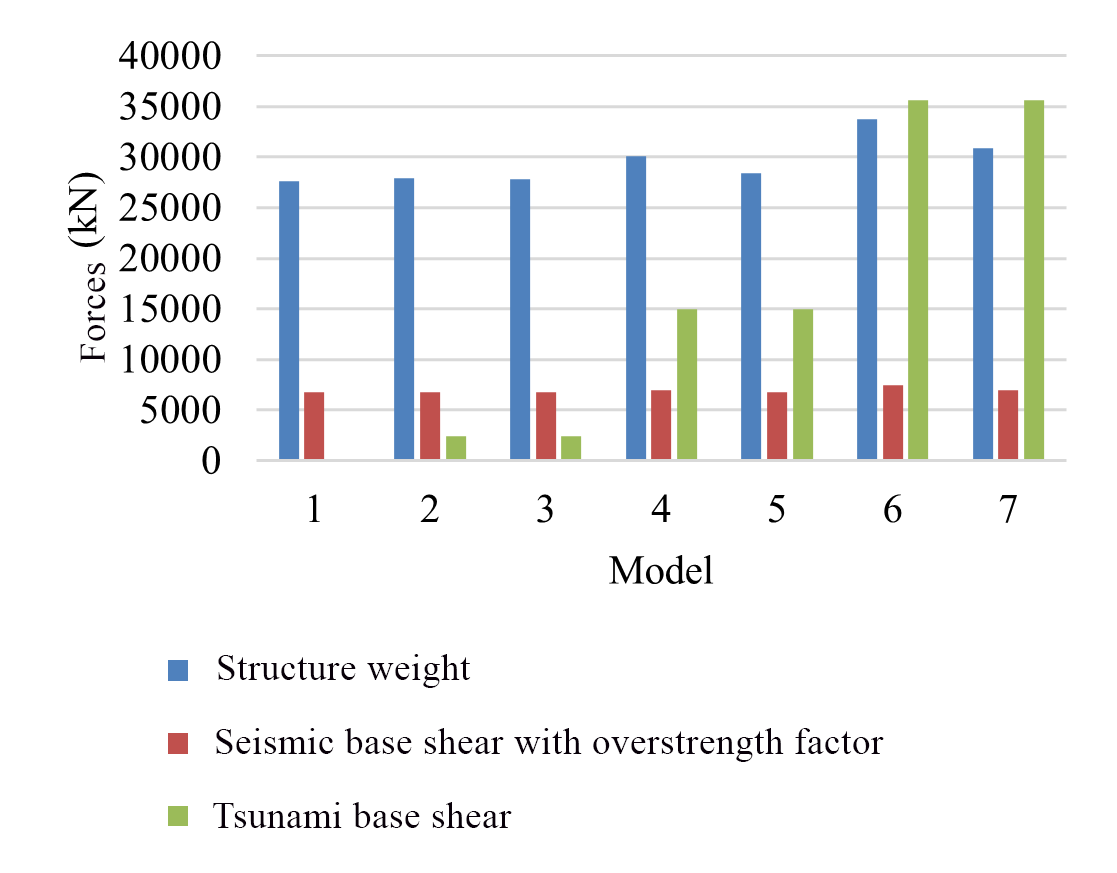
\includegraphics[width=0.7\textwidth]{Picture12_engels.png}
\caption{Structural weight and base shear forces.}
\label{fig:base shear}
\end{figure}

The maximum forces in beams and columns were compared for each model. The forces for the beam elements were reviewed for the case of the overall hydrodynamic load. The internal force for the beam elements was taken for the largest value for each model, for support and middle section values. Figures \ref{fig:maxmomentbeam} and \ref{fig:maxshearbeam} show the maximum values for internal forces in each model for beam structural elements.

\begin{figure}[H]
\centering
\includegraphics[width=0.6\textwidth]{Picture13_engels.png}
\caption{Maximum bending moment for beams in each model.}
\label{fig:maxmomentbeam}
\end{figure}

\begin{figure}[H]
\centering
\includegraphics[width=0.6\textwidth]{Picture14_engels.png}
\caption{Maximum shear force for beams in each model.}
\label{fig:maxshearbeam}
\end{figure}


The internal forces for the columns were taken in the case of component hydrodynamic loads for the exterior and interior columns. The internal forces taken were in the form of axial force, shear force and bending moment. The internal forces taken were for the exterior column and interior column. Figures \ref{fig:maxaxialcolumn} to \ref{fig:maxmomentcolumn} show the plot of internal forces for column structural elements for each model.

\begin{figure}[H]
\centering
\includegraphics[width=0.6\textwidth]{Picture15_engels.png}
\caption{Maximum axial force for columns in each model.}
\label{fig:maxaxialcolumn}
\end{figure}

\begin{figure}[H]
\centering
\includegraphics[width=0.5\textwidth]{Picture16_engels.png}
\caption{Maximum shear force for columns in each model.}
\label{fig:maxshearcolumn}
\end{figure}

\begin{figure}[H]
\centering
\includegraphics[width=0.5\textwidth]{Picture17_engels.png}
\caption{Maximum bending moment for columns in each model.}
\label{fig:maxmomentcolumn}
\end{figure}

For beams, the review was divided into two main sections which were the support and middle section. From figures \ref{fig:maxmomentbeam} and \ref{fig:maxshearbeam} it can be seen that the trend for internal forces from model 2 to model 7 was increasing. The reason was that the lateral load given was increasingly related to tsunami heights. Model 7 experienced a reduction in the force in the beam when compared to model 6. This was due to the reinforcement yielding mechanism that occurred in model 7 which reduced the internal forces. The yielding mechanism could be seen in figure \ref{fig:tsunamidrift}, where the nonlinear model could surpass the limit of linearity imposed by SNI 1727:2020.

\begin{figure}[H]
\centering
\includegraphics[width=0.5\textwidth]{Picture18_engels.png}
\caption{Final drift ratio for each tsunami model.}
\label{fig:tsunamidrift}
\end{figure}

From figures \ref{fig:maxaxialcolumn} to \ref{fig:maxmomentcolumn}, it can be seen that the internal forces due to the impact load of debris have an almost constant magnitude. The debris impact loads also have relatively smaller internal forces than the hydrodynamic loads. This causes the design of structures for high tsunamis to be usually controlled by hydrodynamic loads. The impact load of debris generally controls the design of the upper-floor exterior columns.

Figures \ref{fig:maxshearcolumn} and \ref{fig:maxmomentcolumn} show that the shear forces and bending moments in the exterior columns were much greater than the forces in the interior columns. The bending moment in the nonlinear models was significantly reduced in the exterior column compared to linear models. The biggest moment reduction occurs in model 5 which was equal to \SI{49.66}{\percent} from model 4. This was also due to the distribution of forces on the interior columns in nonlinear models. Trends in interior columns look monotonously rising for both internal forces which means the nonlinear models interior columns contributed more to resist the base shear of tsunami loads compared to linear models.

The net force for the structure in table \ref{tab:recap lifting} shows that the lifting force that occurred was not enough to lift the structure. This means that the foundation did not need to be designed against uplift. The smallest net force that occurs is \num{155.76} \si{kN} (downward) in the interior column of model 5 (2 floors tsunami with nonlinear acceptance criteria).

\renewcommand{\arraystretch}{1}
\begin{longtable}{P{0.5in} P{1in} P{1in} P{1in} P{1in}}
\caption{Summary of critical axial forces in base columns to determine lifting.}\\
\headrow \thead{Model} & \thead{Interior column (kN)} & \thead{Middle exterior column (kN)} & \thead{Corner exterior column (kN)} & \thead{Conclusion} \\
2 & $-504.07$ & $-618.97$ & $-528.01$ & No lifting occured \\
3 & $-501.67$ & $-622.72$ & $-534.52$ & No lifting occured \\
4 & $-262.26$ & $-497.11$ & $-460.46$ & No lifting occured \\
5 & $-155.76$ & $-428.88$ & $-416.76$ & No lifting occured \\
6 & $-321.36$ & $-399.90$ & $-345.58$ & No lifting occured \\
7 & $-344.96$ & $-387.64$ & $-360.95$ & No lifting occured \\
\label{tab:recap lifting}
\end{longtable}

Nonlinear plastic hinges were compared to nonlinear models 3, 5 and 7. The results of the plastic hinges showed that all structures exhibited the highest nonlinear condition on B-IO \footnote{B-IO refers to immediate occupancy (IO) hinges which means there are minor damages to the structure. For more in-depth information, please refer to \citep{asceretro}.} \enlargethispage{-\baselineskip}. The plastic hinges that occurred varied between the three models. In model 3 there are 9 plastic hinges, model 5 has 73 plastic hinges and model 7 has a total of 152 plastic hinges.

\begin{figure}[H]
\centering
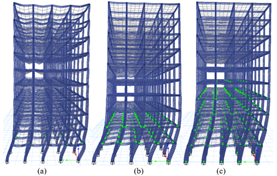
\includegraphics[width=0.6\textwidth]{Picture19.png}
\caption{Distribution of plastic hinges.}
\label{fig:plastichinges}
\end{figure}

\section{Conclusion}
\label{sec:conclusion}
\begin{enumerate}
\item{The internal forces due to the earthquake had a comparable magnitude to the force in the beam due to the tsunami loads. The forces in the beam due to the earthquake were exceeded in a 3-story high tsunami. For example, the support bending moment of model 1 (earthquake only) had a magnitude of \num{-80.56} \si{kN.m} for negative bending moments, this value had only been exceeded in model 6 which had a value of \num{-123.60} \si{kN.m}. Meanwhile, internal forces in the column had a magnitude that far exceeds the internal forces due to the earthquake loads, especially for shear forces and bending moments. Acceptance of the structure in models 2 to 7 also affects the internal forces that occur. Acceptance of nonlinear models can reduce the bending moment that occurs in the column up to \SI{49.66}{\percent} compared to the linear models.}

\item{The lifting force that occurred had not been able to lift the structure as a whole. The most significant net force was \num{155.76} \si{kN} (downward). This smallest net force occurred in the interior column of model 5 (2-story tsunami with nonlinear acceptance criteria). This indicated that the weight of the structure was able to counteract the lifting force that occurred.}

\item{The inundation height has an effect on the hydrodynamic force. The higher the tsunami, the greater the hydrodynamic force. The magnitude of the tsunami base shear force on the models with inundation height of 1 floor, 2 floors and 3 floors respectively were \num{2400.64} \si{kN}; \num{15003.99} \si{kN}; \num{35600.49} \si{kN}. The increase in the base shear force occurs exponentially because the magnitude of the force depends on the square of the velocity with the upper limit of \num{15.20} \si{m/s}. The maximum bending moment that occurs in the exterior column on the models with tsunami as height as 1 floor, 2 floors and 3 floors respectively were \num{680.52} \si{kN.m}; \num{3086.75} \si{kN.m}; and \num{6629.72} \si{kN.m}. These internal forces increase significantly in relation to the tsunami height of each model.
}

\item{The tsunami load affects the design of structural elements up to the tsunami height. Structural elements that are above the inundation level are generally not affected by the tsunami that occurs. The upper-floor exterior columns were generally controlled by debris impact loads. The lower-column were controlled by hydrodynamic loads. The weight of all models differs from the earthquake model (model 1). The largest structural weight was in model 6 (3-floor tsunami with linear acceptance criteria) which was \num{33746.46} \si{kN} or an increase of \SI{22.03}{\percent} from model 1.}
\end{enumerate}

%\begin{figure}
%\begin{minipage}{0.47\textwidth}
%\includegraphics[width=\linewidth]{example-image}
%\subcaption{This is a subfigure}
%\end{minipage}
%\hfill
%\begin{minipage}{0.47\textwidth}
%\includegraphics[width=\linewidth]{example-image}
%\subcaption{This is another subfigure}
%\end{minipage}
%
%\caption{This is a caption for the entire figure}
%\label{fig:twosubs}
%\end{figure}

%\blinddocument

\bigskip

\paragraph*{Acknowledgments.} This paper was made to fulfill one of the requirements to finish the bachelor's degree in Civil Engineering and Planning at Sriwijaya University.

\paragraph*{Data Availability Statement.} Code for part of structural modeling can be found on \url{https://github.com/sanlocoz/structural-modeling}. Data will be made available by requests.

\nocite{*}
\printbibliography
\end{document}
